\section{Disaggregated Computing}
\label{ch:background:disaggregated}



\begin{figure}[t]
  \centering
    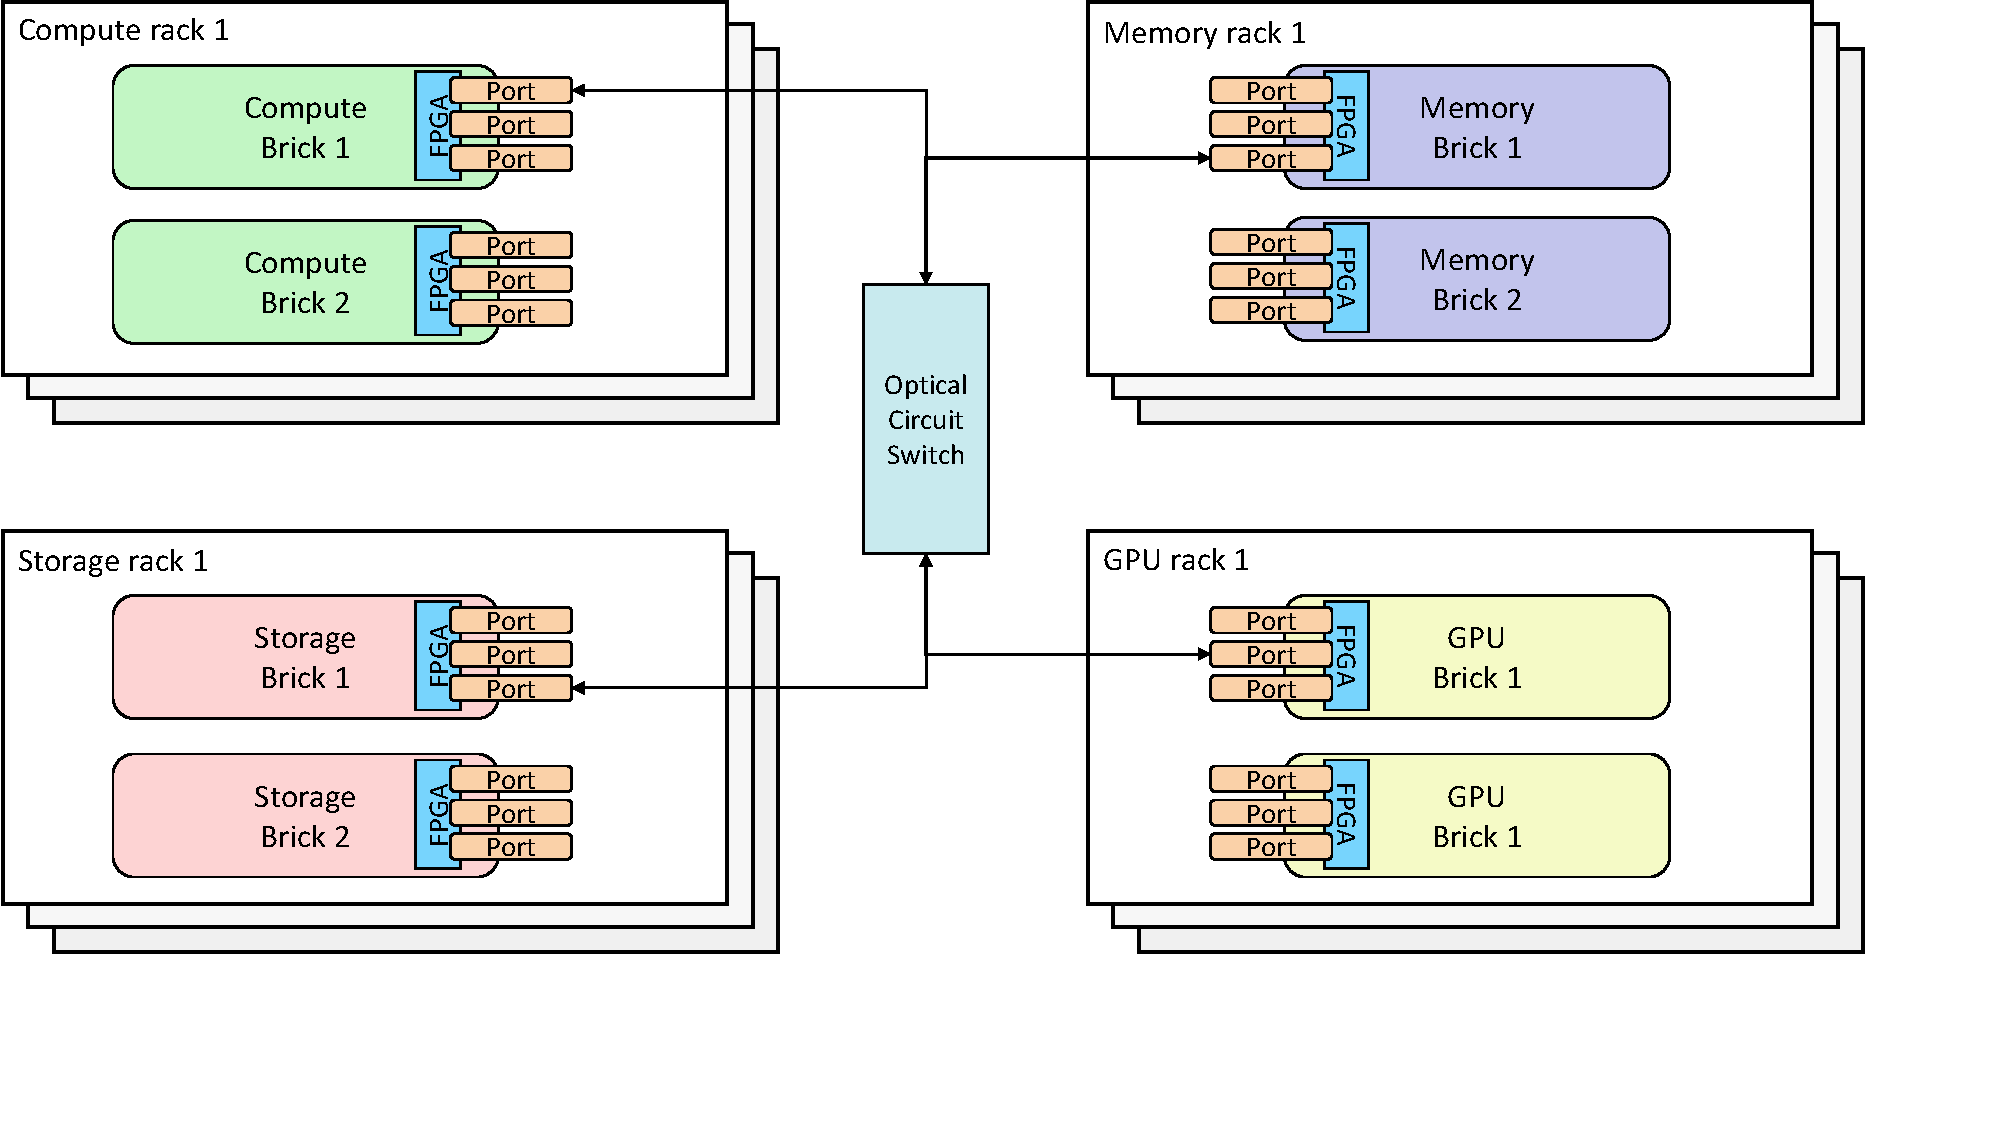
\includegraphics[trim={0 2cm 2cm 0},clip,width=\linewidth]{chapters/background/figures/disaggregated.pdf}
    \caption[Disaggregated architecture similar to dReDBox project]{\textbf{Disaggregated architecture similar to dReDBox project~\cite{dis1}.} The figure shows an example disaggregated architecture similar to dReDBox project~\cite{dis1} that are common in modern data centers. Rather than fully-fledged computers, the architecture employs different racks - compute, memory, storage etc. Inside this racks, there are multiple special purpose SoC-based microservers that are called bricks. These bricks have communication ports to talk to other bricks over fast optical circuit switches.}
    \label{fig:disagg_bg}
\end{figure}
